\begin{enumerate}[label=\thesubsection.\arabic*,ref=\thesubsection.\theenumi]
\item  Equal chords of a circle  are equidistant from the centre.
	\\
		\solution 
	In \figref{fig:ncert-circ-1},	
\begin{align}
	l &= 2r\sin \frac{\theta_1}{2}
	= 2r\sin \frac{\theta_2}{2}
	\\
	\implies \theta_1 &= \theta_2 = \theta
\end{align}
Thus, the distances
\begin{align}
	d_1 = r \cos \frac{\theta}{2} = d_2.
\end{align}
\begin{figure}[H]
	\begin{center}
		{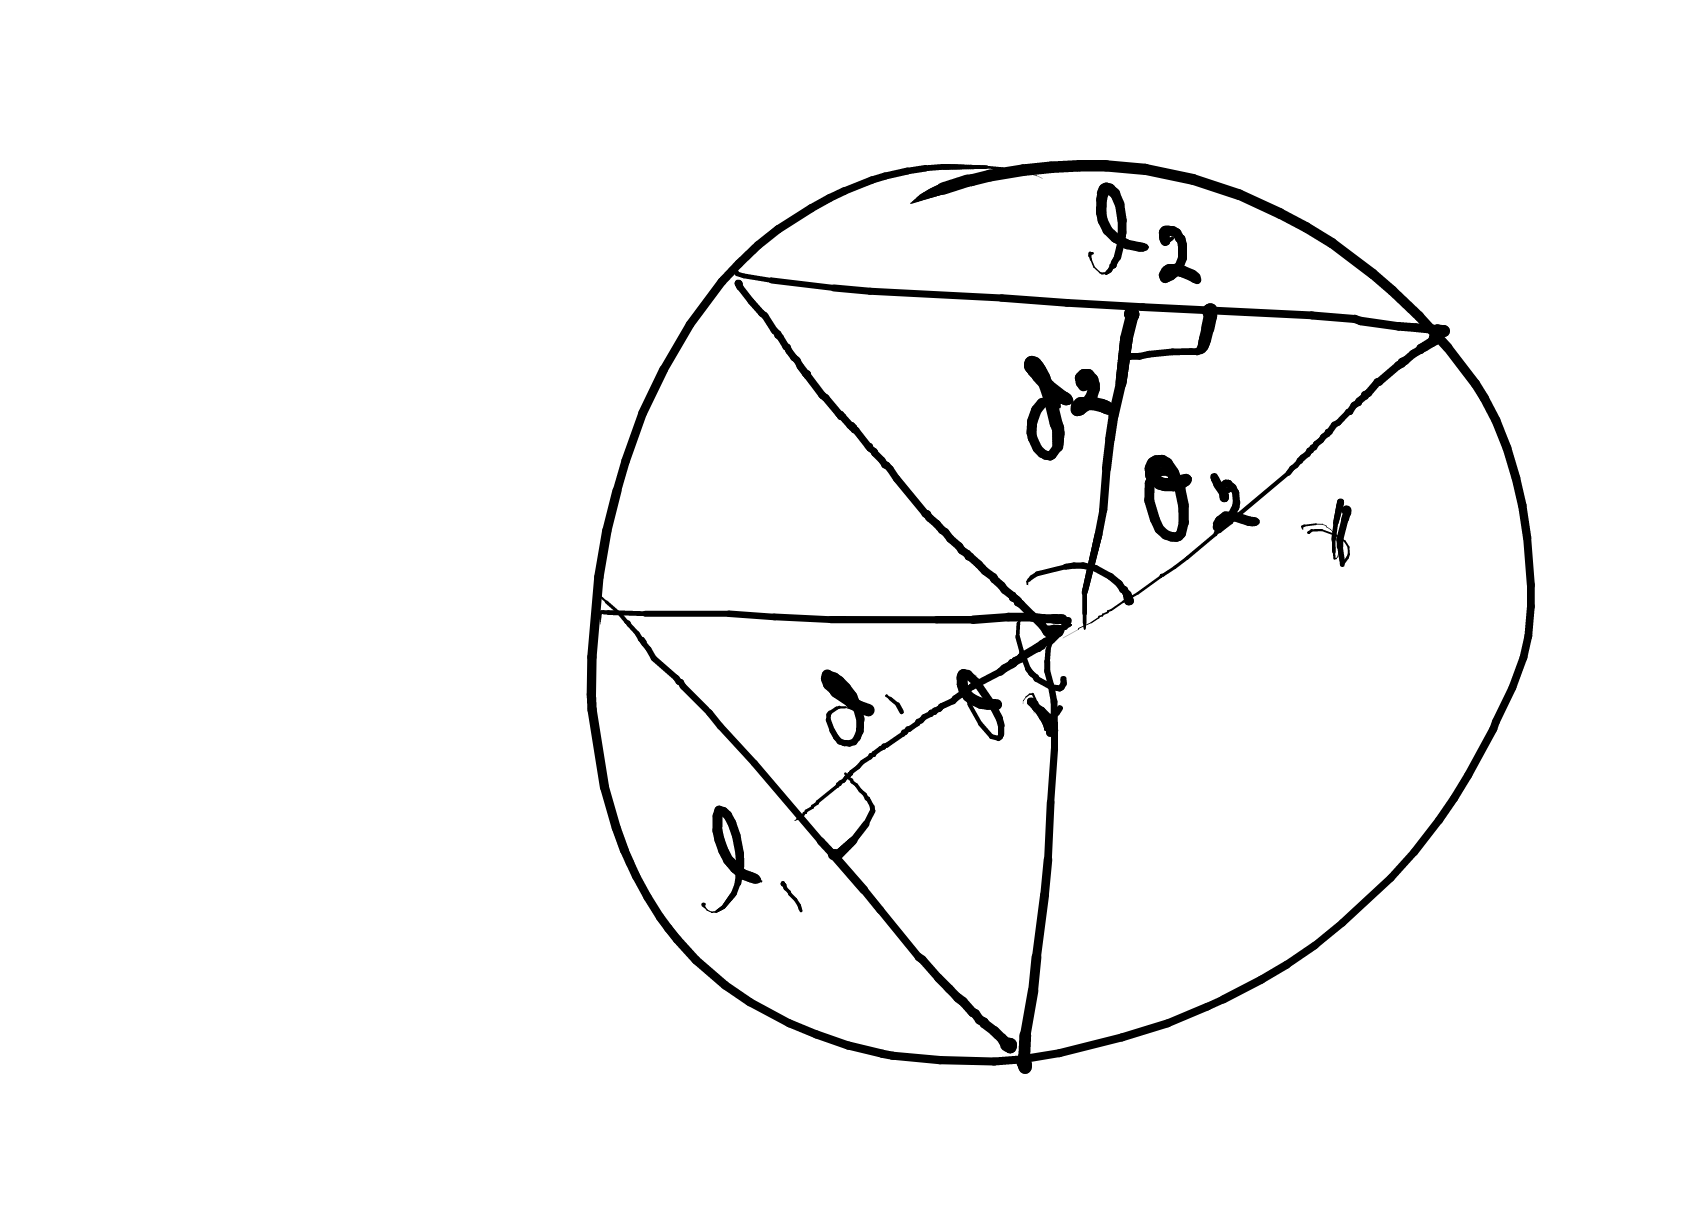
\includegraphics[width=0.6\columnwidth]{figs/ncert/circle/1.png}}
	\end{center}
	\caption{}
	\label{fig:ncert-circ-1}	
\end{figure}
%
 \item  Angle in a semicircle is a right angle. 
	\\
		\solution 
	In \figref{fig:ncert-circ-2}, considering a unit circle	
	with
\begin{align}
	\vec{A}&= \myvec{\cos \theta \\ \sin \theta}\,
	\vec{B}= \myvec{-1 \\ 0}\,
	\vec{C}= \myvec{1 \\ 0}
	\\
	\brak{A-B}^{\top}
	\brak{A-C}^{\top}
	&=
	 \myvec{\cos \theta+1 & \sin \theta}
\myvec{\cos \theta -1 \\ \sin \theta}
\\
	&=\cos^2\theta -1 + \sin^2\theta = 0
\end{align}
Thus, $AB \perp AC$.
\begin{figure}[H]
	\begin{center}
		{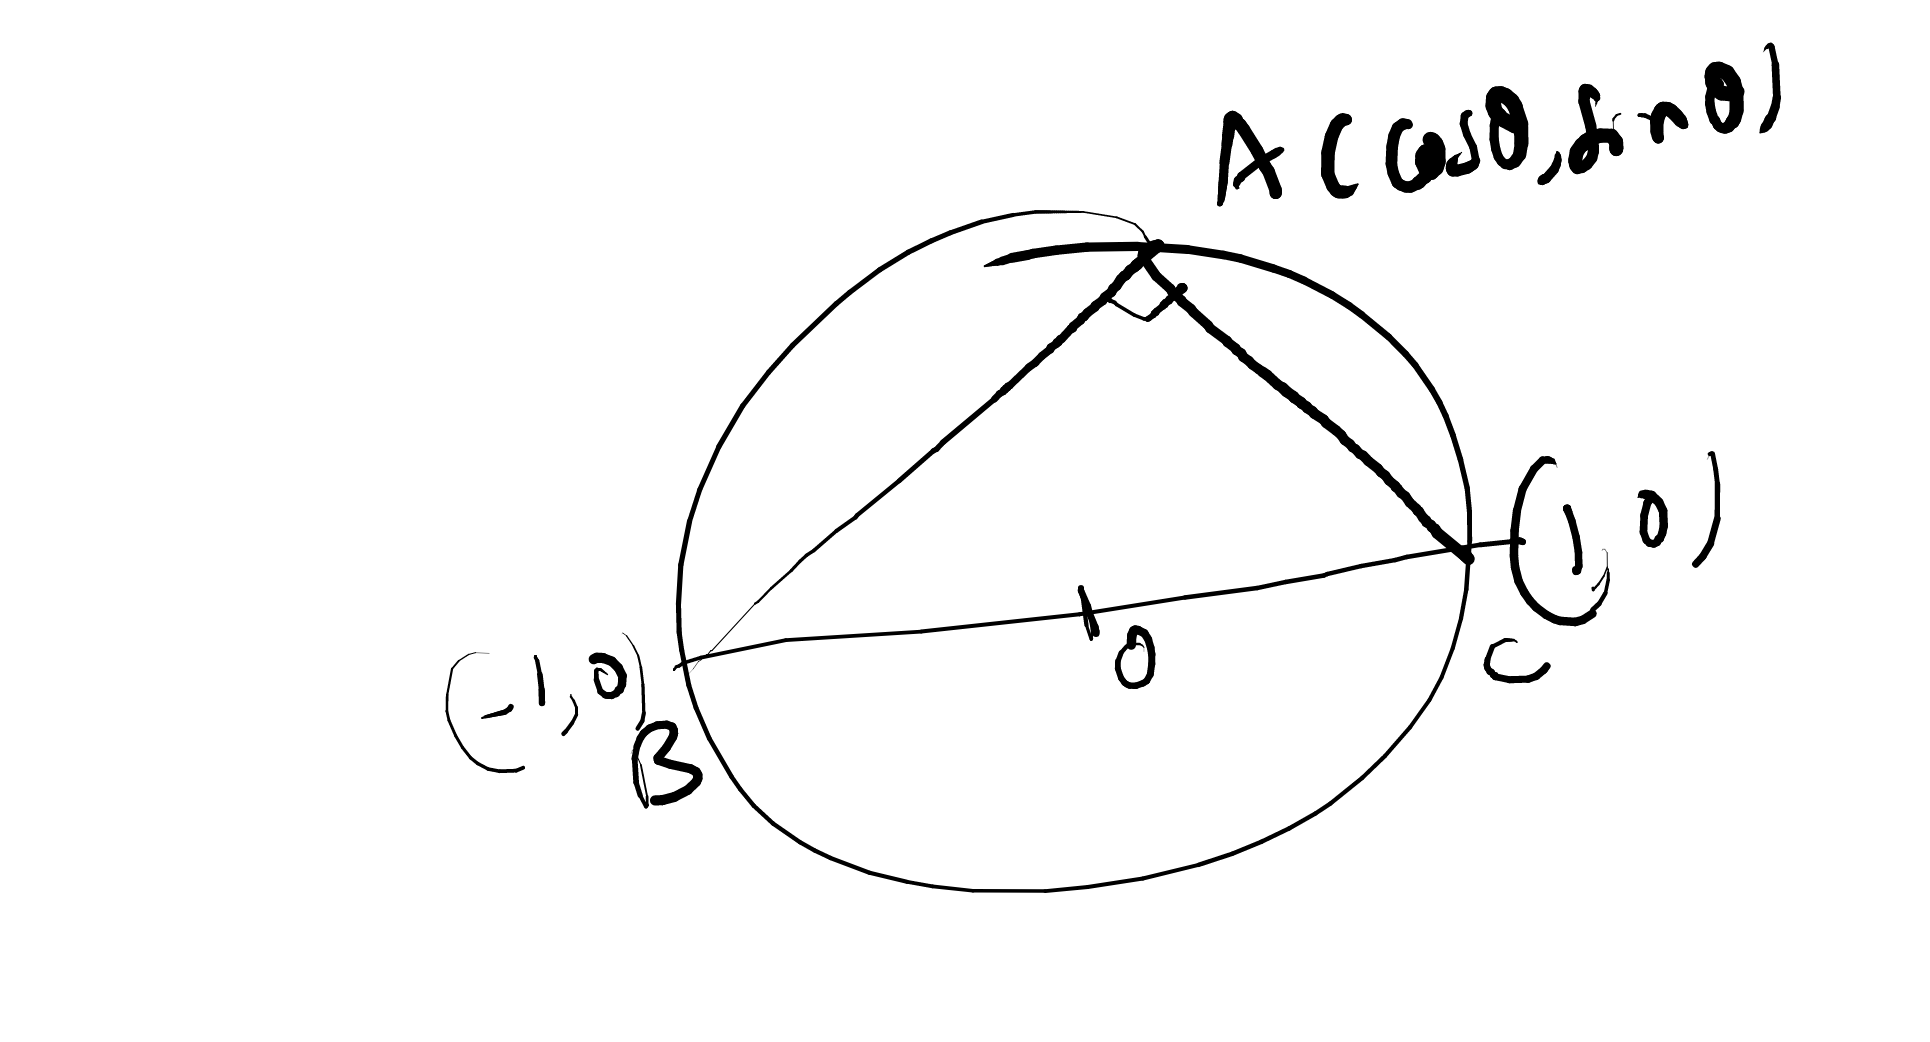
\includegraphics[width=0.6\columnwidth]{figs/ncert/circle/2.png}}
	\end{center}
	\caption{}
	\label{fig:ncert-circ-2}	
\end{figure}
%
%
\item Two circles of radii 5 cm and 3 cm intersect at two points and the distance between their centres is 4 cm. Find the length of the common chord.
	\\
		\solution 
	In \figref{fig:ncert-circ-3}, 
\begin{align}
	\cos \alpha &= \frac{r_1^2+d^2-r_2^2}{2r_1r_2} = 0.8
	\\
\implies	l &= 2r_1\sin \alpha = 6
\end{align}
upon substituting numerical values.
\begin{figure}[H]
	\begin{center}
		{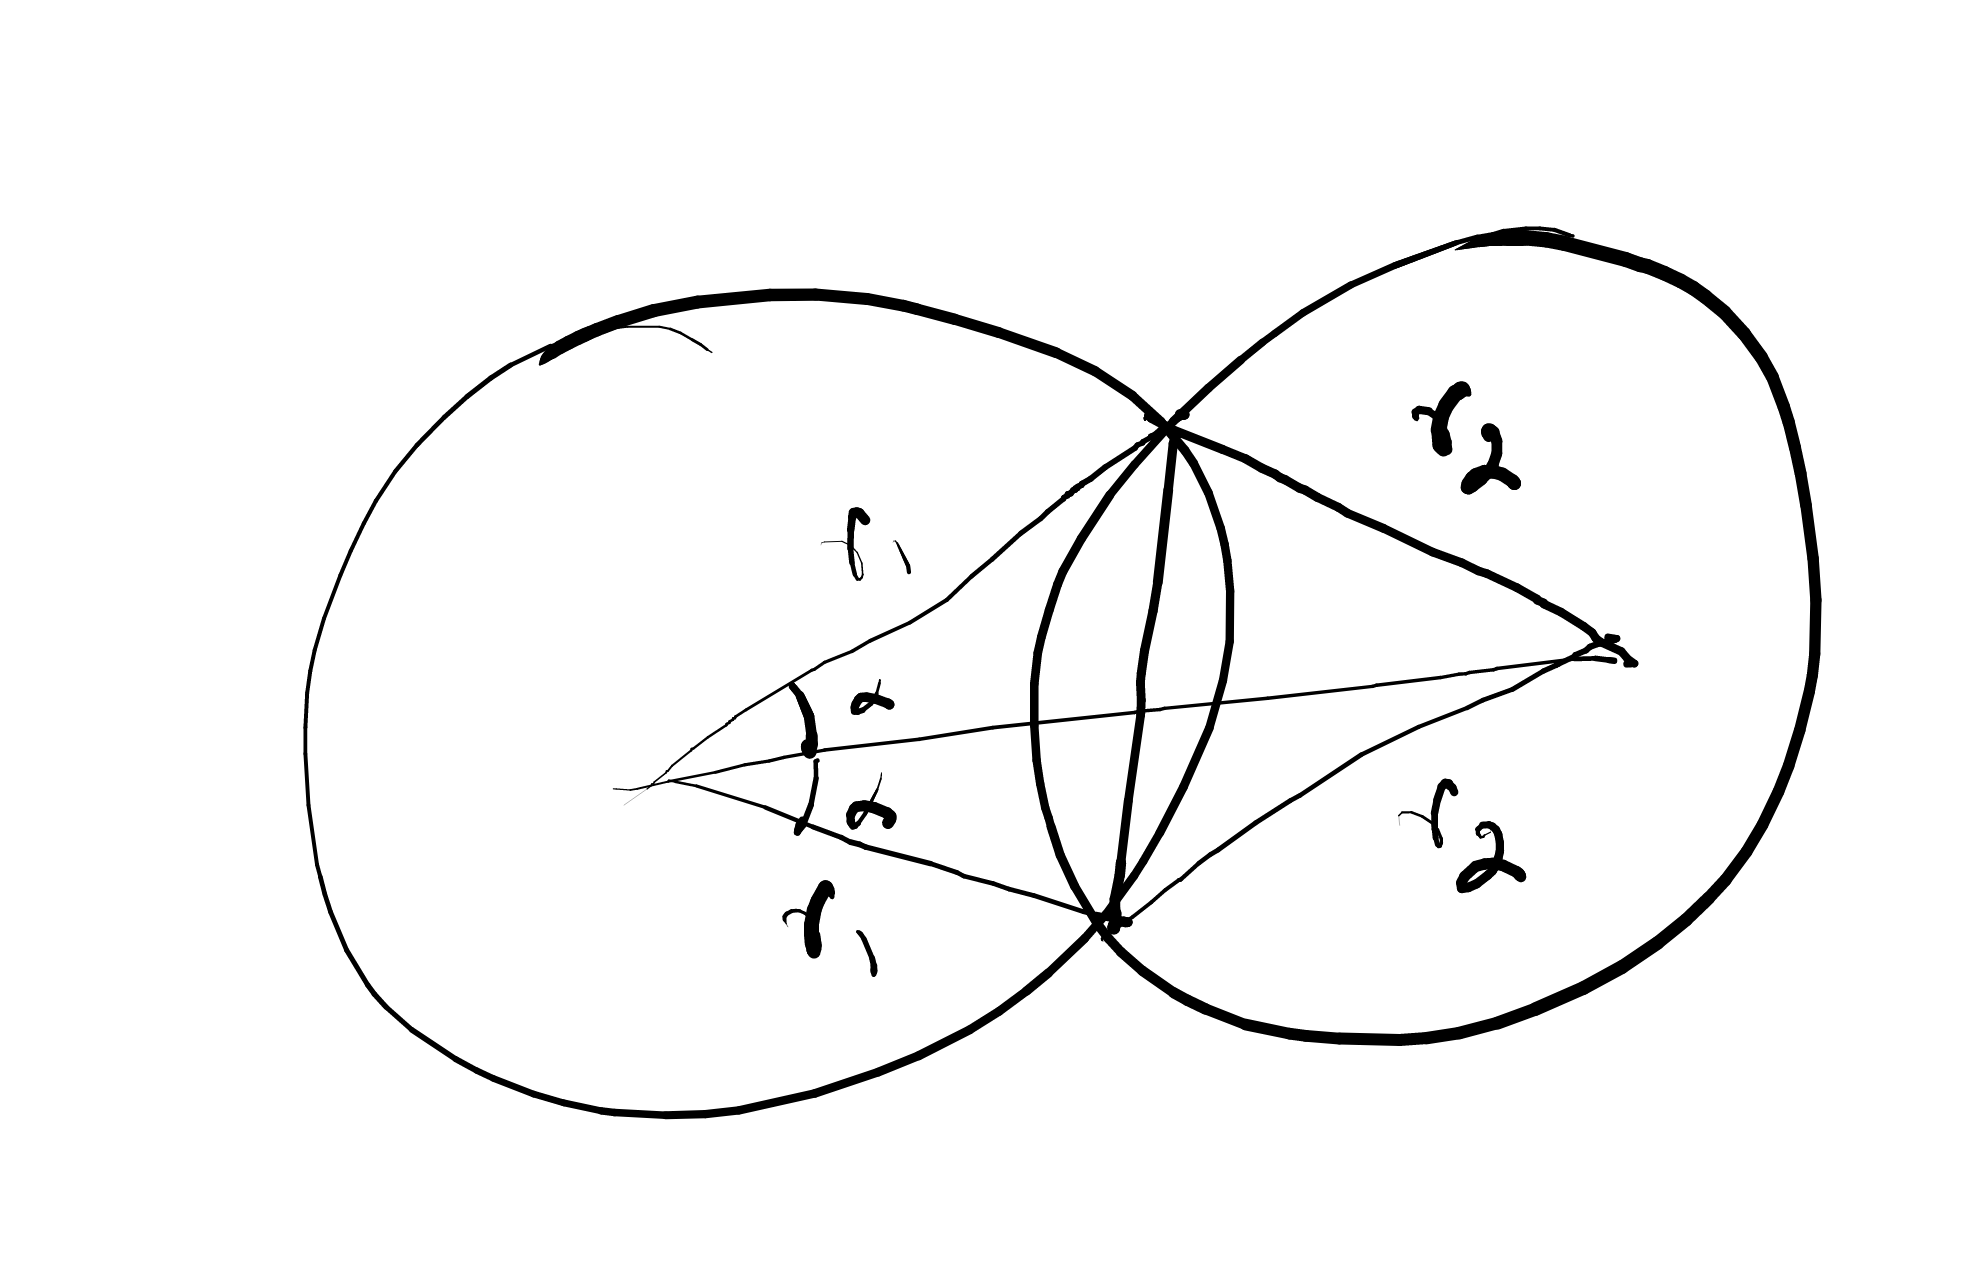
\includegraphics[width=0.6\columnwidth]{figs/ncert/circle/3.png}}
	\end{center}
	\caption{}
	\label{fig:ncert-circ-3}	
\end{figure}
%
\item Two chords $AB$ and $CD$ of lengths 5 cm and 11 cm respectively of a circle are parallel
to each other and are on opposite sides of its centre. If the distance between $AB$ and
$CD$ is 6 cm, find the radius of the circle.
	\\
		\solution 
	In \figref{fig:ncert-circ-4}, 
\begin{align}
	l_1&=2r \sin \theta_1\,
	l_2=2r \sin \theta_2
	\\
	d &= r \brak{\cos \theta_1+\cos \theta_2}
\end{align}
yielding
\begin{align}
	2d &=  \sqrt{4r^2-l_1^2}+\sqrt{4r^2-l_2^2}
	\\
	\implies 
	\brak{2d -  \sqrt{4r^2-l_1^2}}^2&=4r^2-l_2^2
	\\
	\text{or, }4d^2 -l_1^2+l_2^2&=4d\sqrt{4r^2-l_1^2}
	\\
	\implies r &= \frac{\sqrt{\brak{\frac{4d^2 -l_1^2+l_2^2}{4d}}^2+l_1^2}}{2} = 5.59 
\end{align}
upon substituting numerical values.
\begin{figure}[H]
	\begin{center}
		{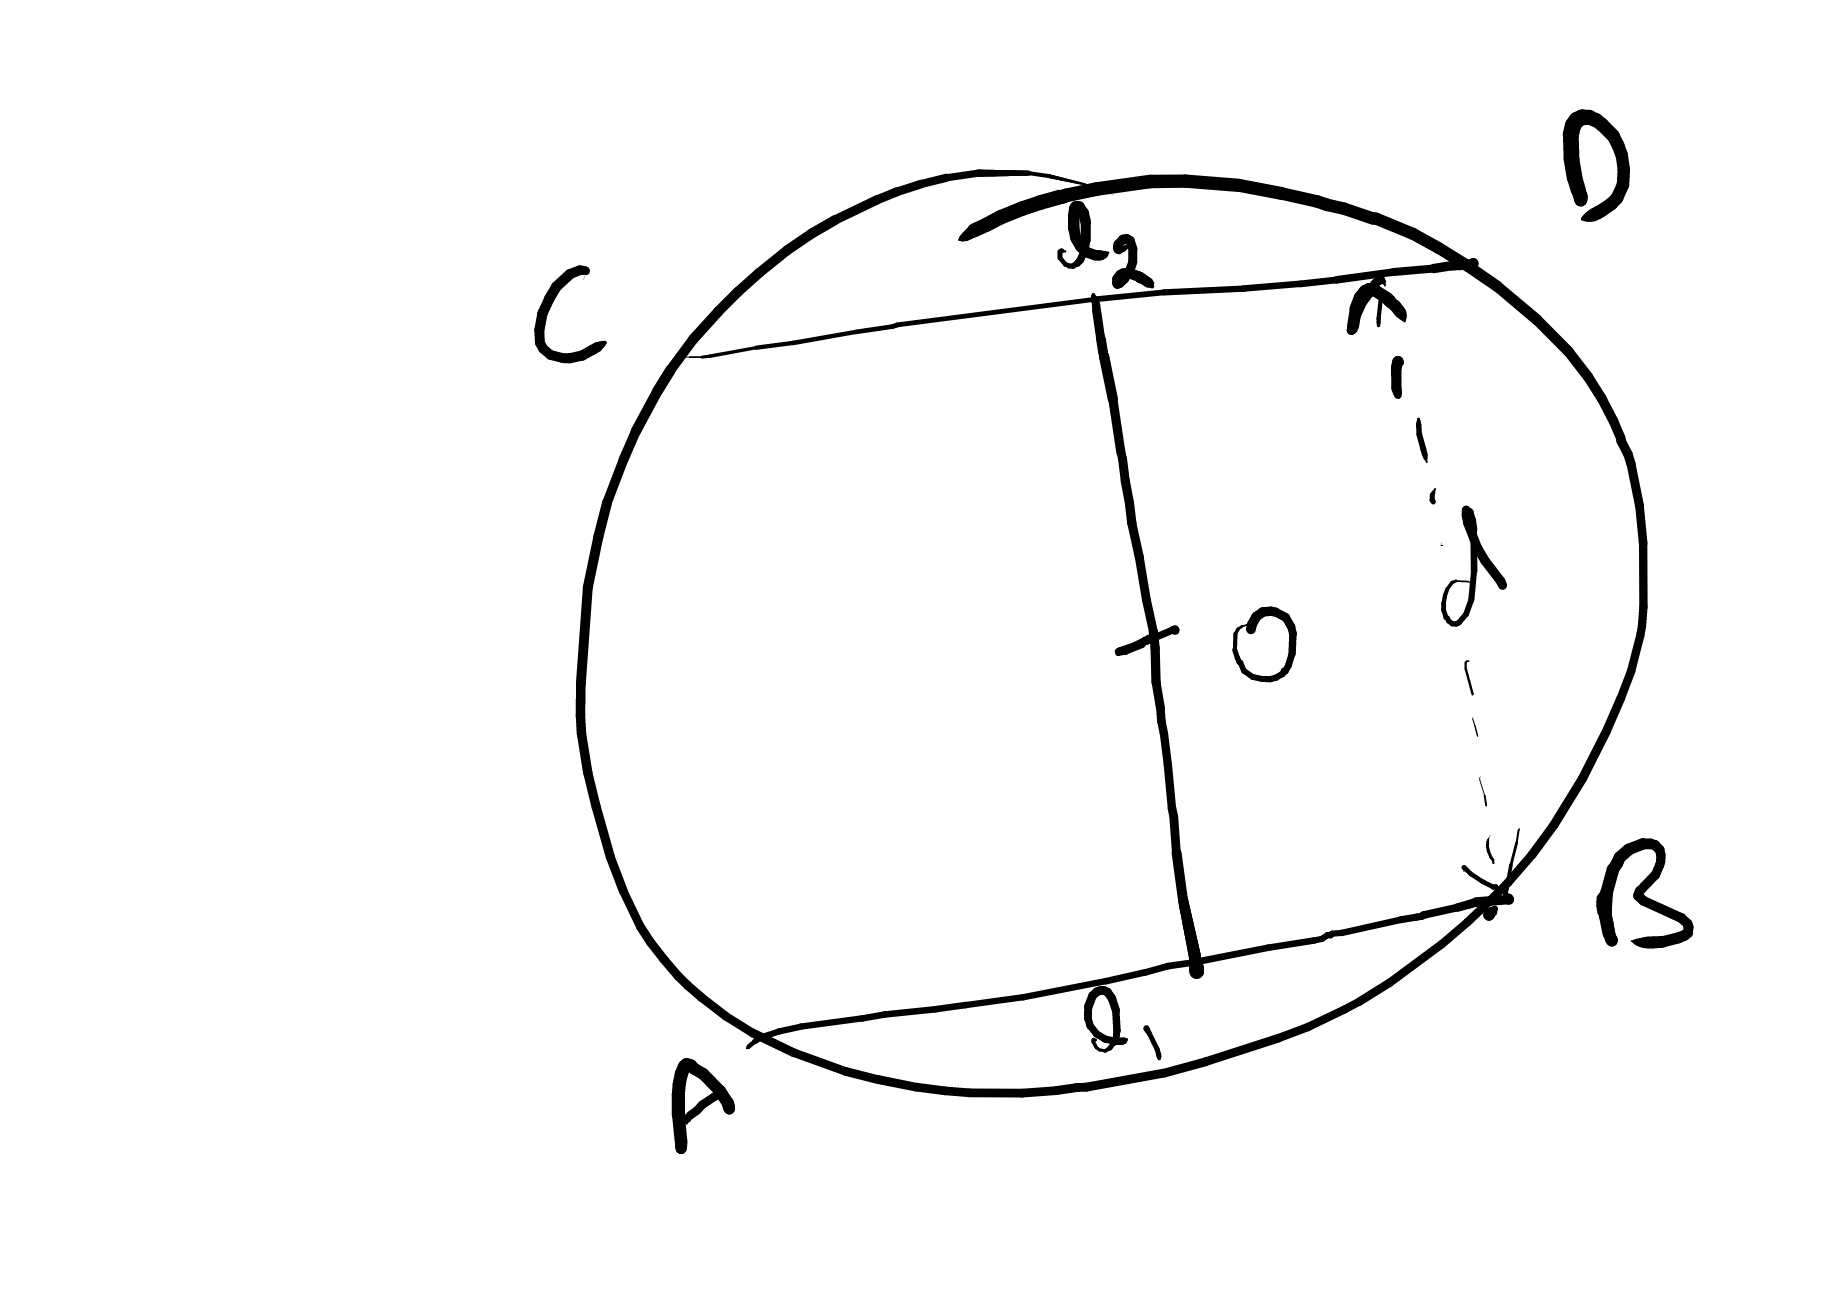
\includegraphics[width=0.6\columnwidth]{figs/ncert/circle/4.png}}
	\end{center}
	\caption{}
	\label{fig:ncert-circ-4}	
\end{figure}
%
\item The lengths of two parallel chords of a circle are 6 cm and 8 cm. If the smaller chord is
at distance 4 cm from the centre, what is the distance of the other chord from the
centre?
\\
\solution
	In \figref{fig:ncert-circ-5}, 
\begin{align}
	l_1&=2r \sin \theta_1\,
	l_2=2r \sin \theta_2
	\\
	d_1 &= r \cos \theta_1\,
	d_2 =r\cos \theta_2
\end{align}
yielding
\begin{align}
	\theta_1 &= \tan^{-1}\brak{\frac{l_1}{2d_1}}
	\\
	\theta_2 &= \sin^{-1}\brak{\frac{l_2\cos \theta_1}{2d_1}}	
	\\
	\implies d_2 &= \frac{l_2}{2}\cot\theta_2 = 3
\end{align}
upon substituting numerical values.
\begin{figure}[H]
	\begin{center}
		{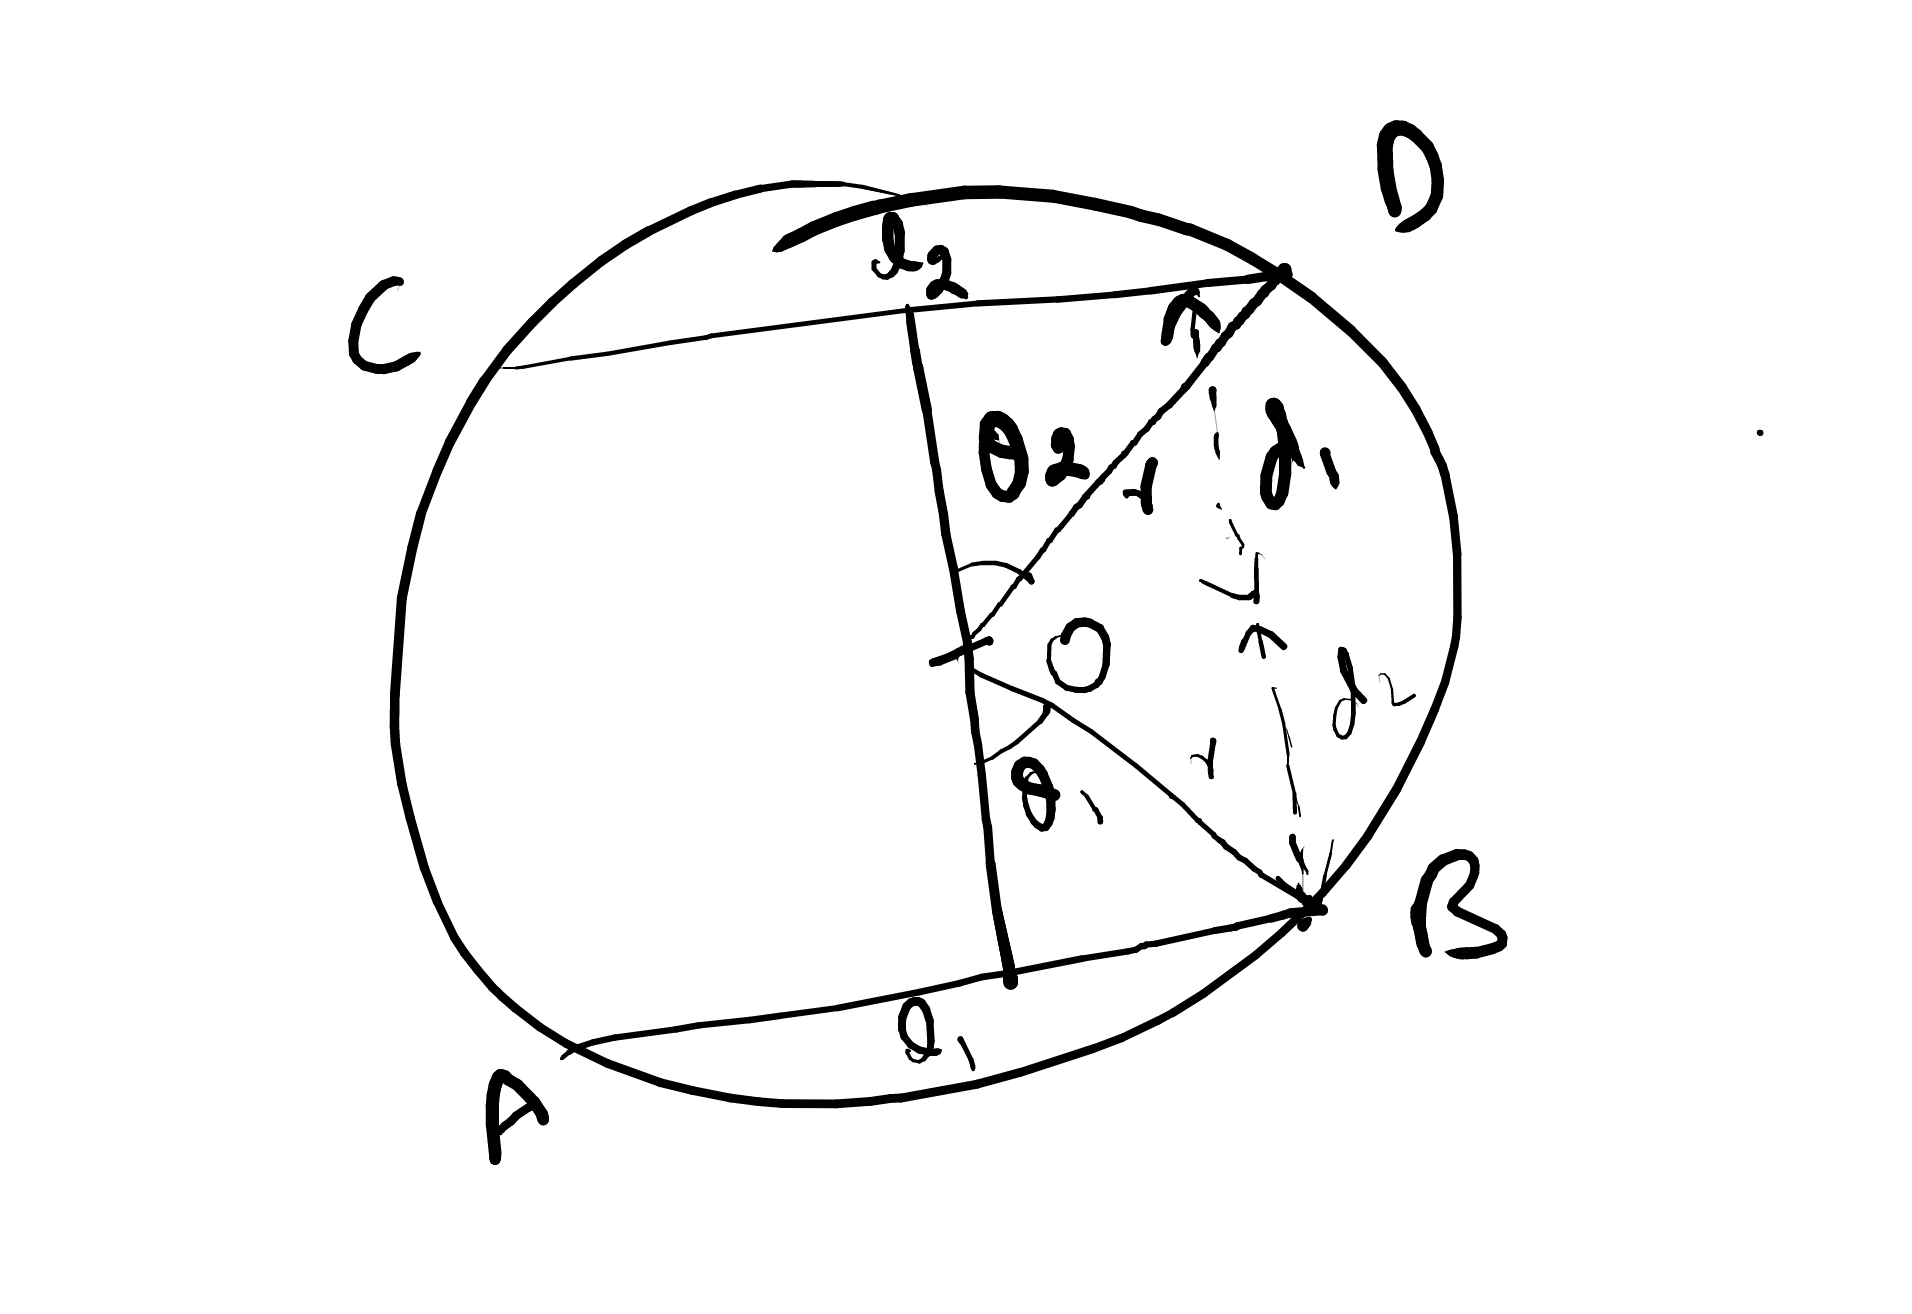
\includegraphics[width=0.6\columnwidth]{figs/ncert/circle/5.png}}
	\end{center}
	\caption{}
	\label{fig:ncert-circ-5}	
\end{figure}
%
\item  Two concentric circles are of radii 5 cm and 3 cm. Find the length of the chord of the larger circle which touches the smaller circle.
\\
\solution
	In \figref{fig:ncert-circ-6}, 
\begin{align}
	\theta &= \cos^{-1}\brak{\frac{r_2}{r_1}}
	\\
\implies	l &= 2r_1\sin \theta = 8
\end{align}
upon substituting numerical values.
\begin{figure}[H]
	\begin{center}
		{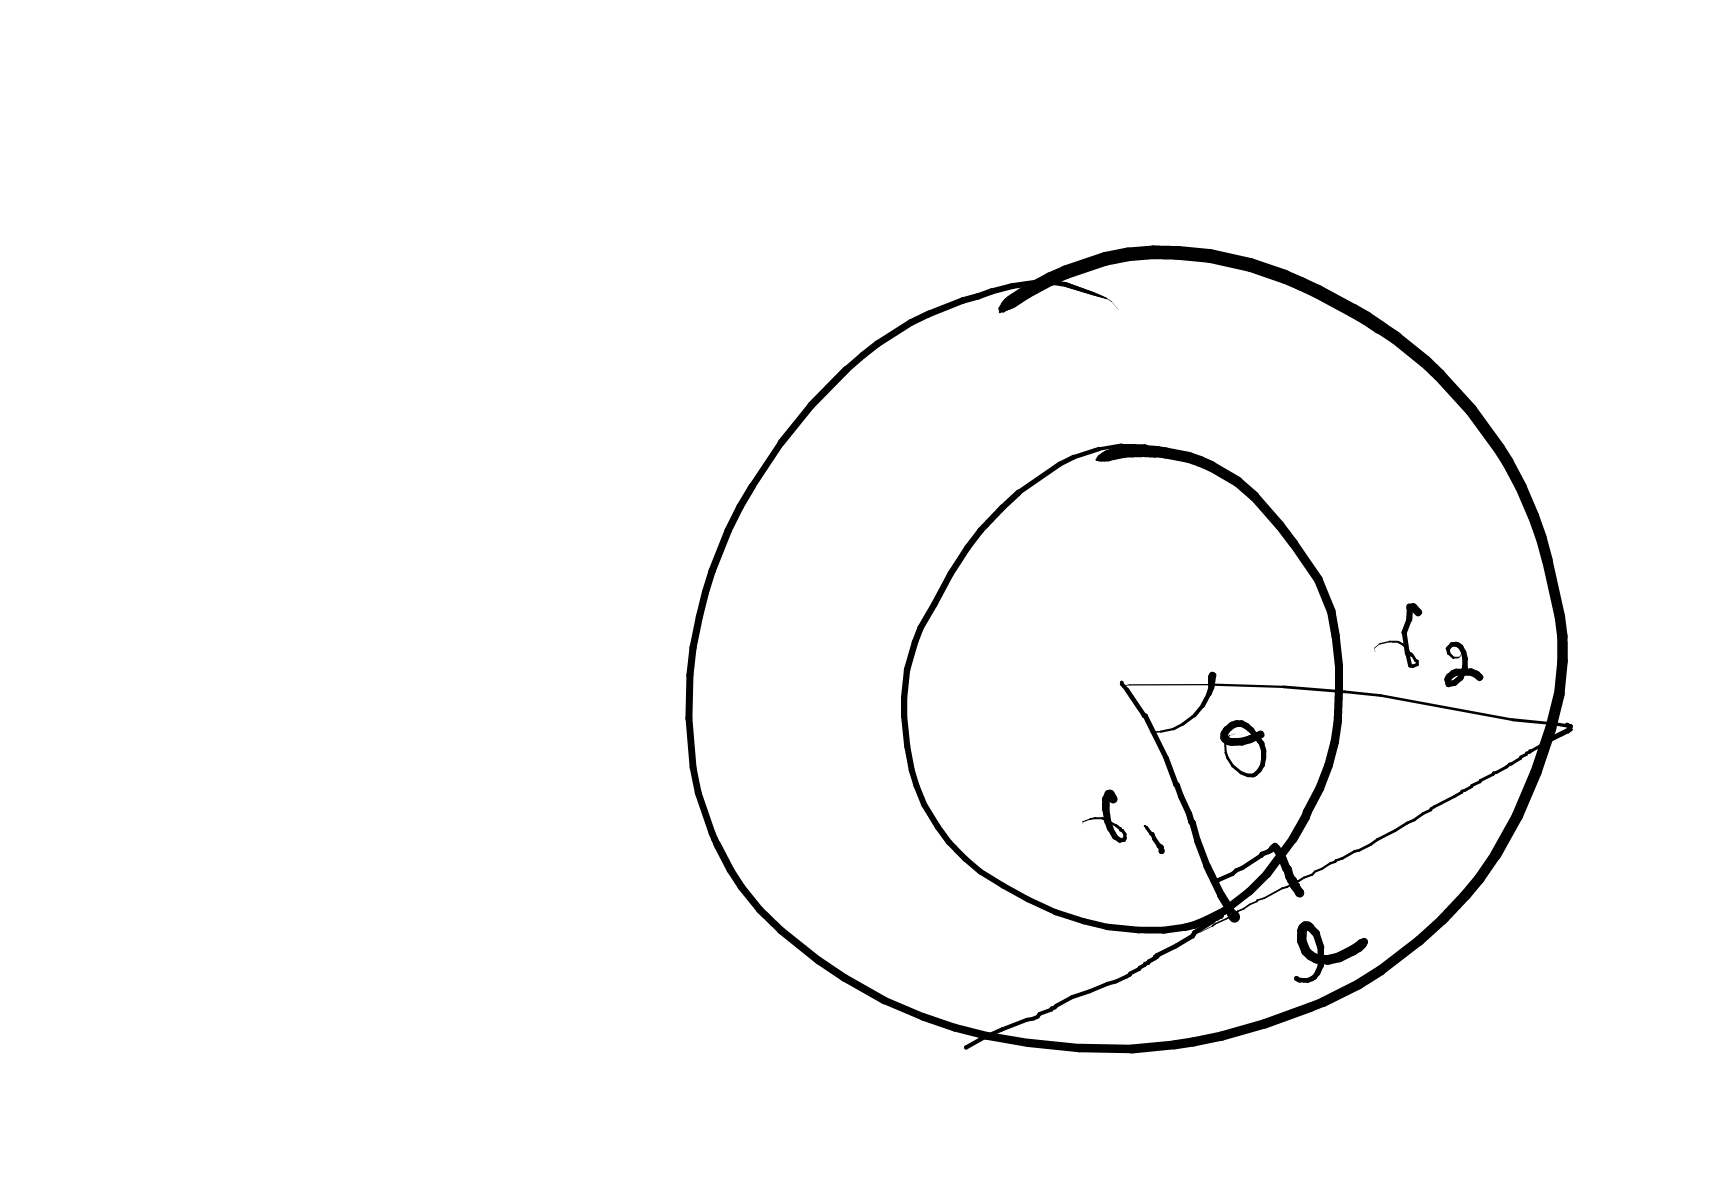
\includegraphics[width=0.6\columnwidth]{figs/ncert/circle/6.png}}
	\end{center}
	\caption{}
	\label{fig:ncert-circ-6}	
\end{figure}
%
\item A $\triangle ABC$ is drawn to circumscribe a circle of radius 4 cm such that the segments $BD$ and $DC$ into which $BC$ is divided by the point of contact $D$ are of lengths 8 cm and 6 cm respectively. Find the sides $AB$ and $AC$.
\\
\solution
	In \figref{fig:ncert-circ-7}, 
\begin{align}
	a &= a_1+a_2
	\frac{B}{2} &= \tan^{-1}\frac{r}{a_1}
	\implies B = 2\tan^{-1}\frac{r}{a_1}
	\\
	\frac{C}{2} &= \tan^{-1}\frac{r}{a_2}
	\implies C = 2\tan^{-1}\frac{r}{a_2}
	\\
	\text{and } A = \pi - B-C
\end{align}
Using sine formula,
\begin{align}
	b = a\frac{\sin B}{\sin A}=13\,
	c = a\frac{\sin C}{\sin A}=15
\end{align}
\begin{figure}[H]
	\begin{center}
		{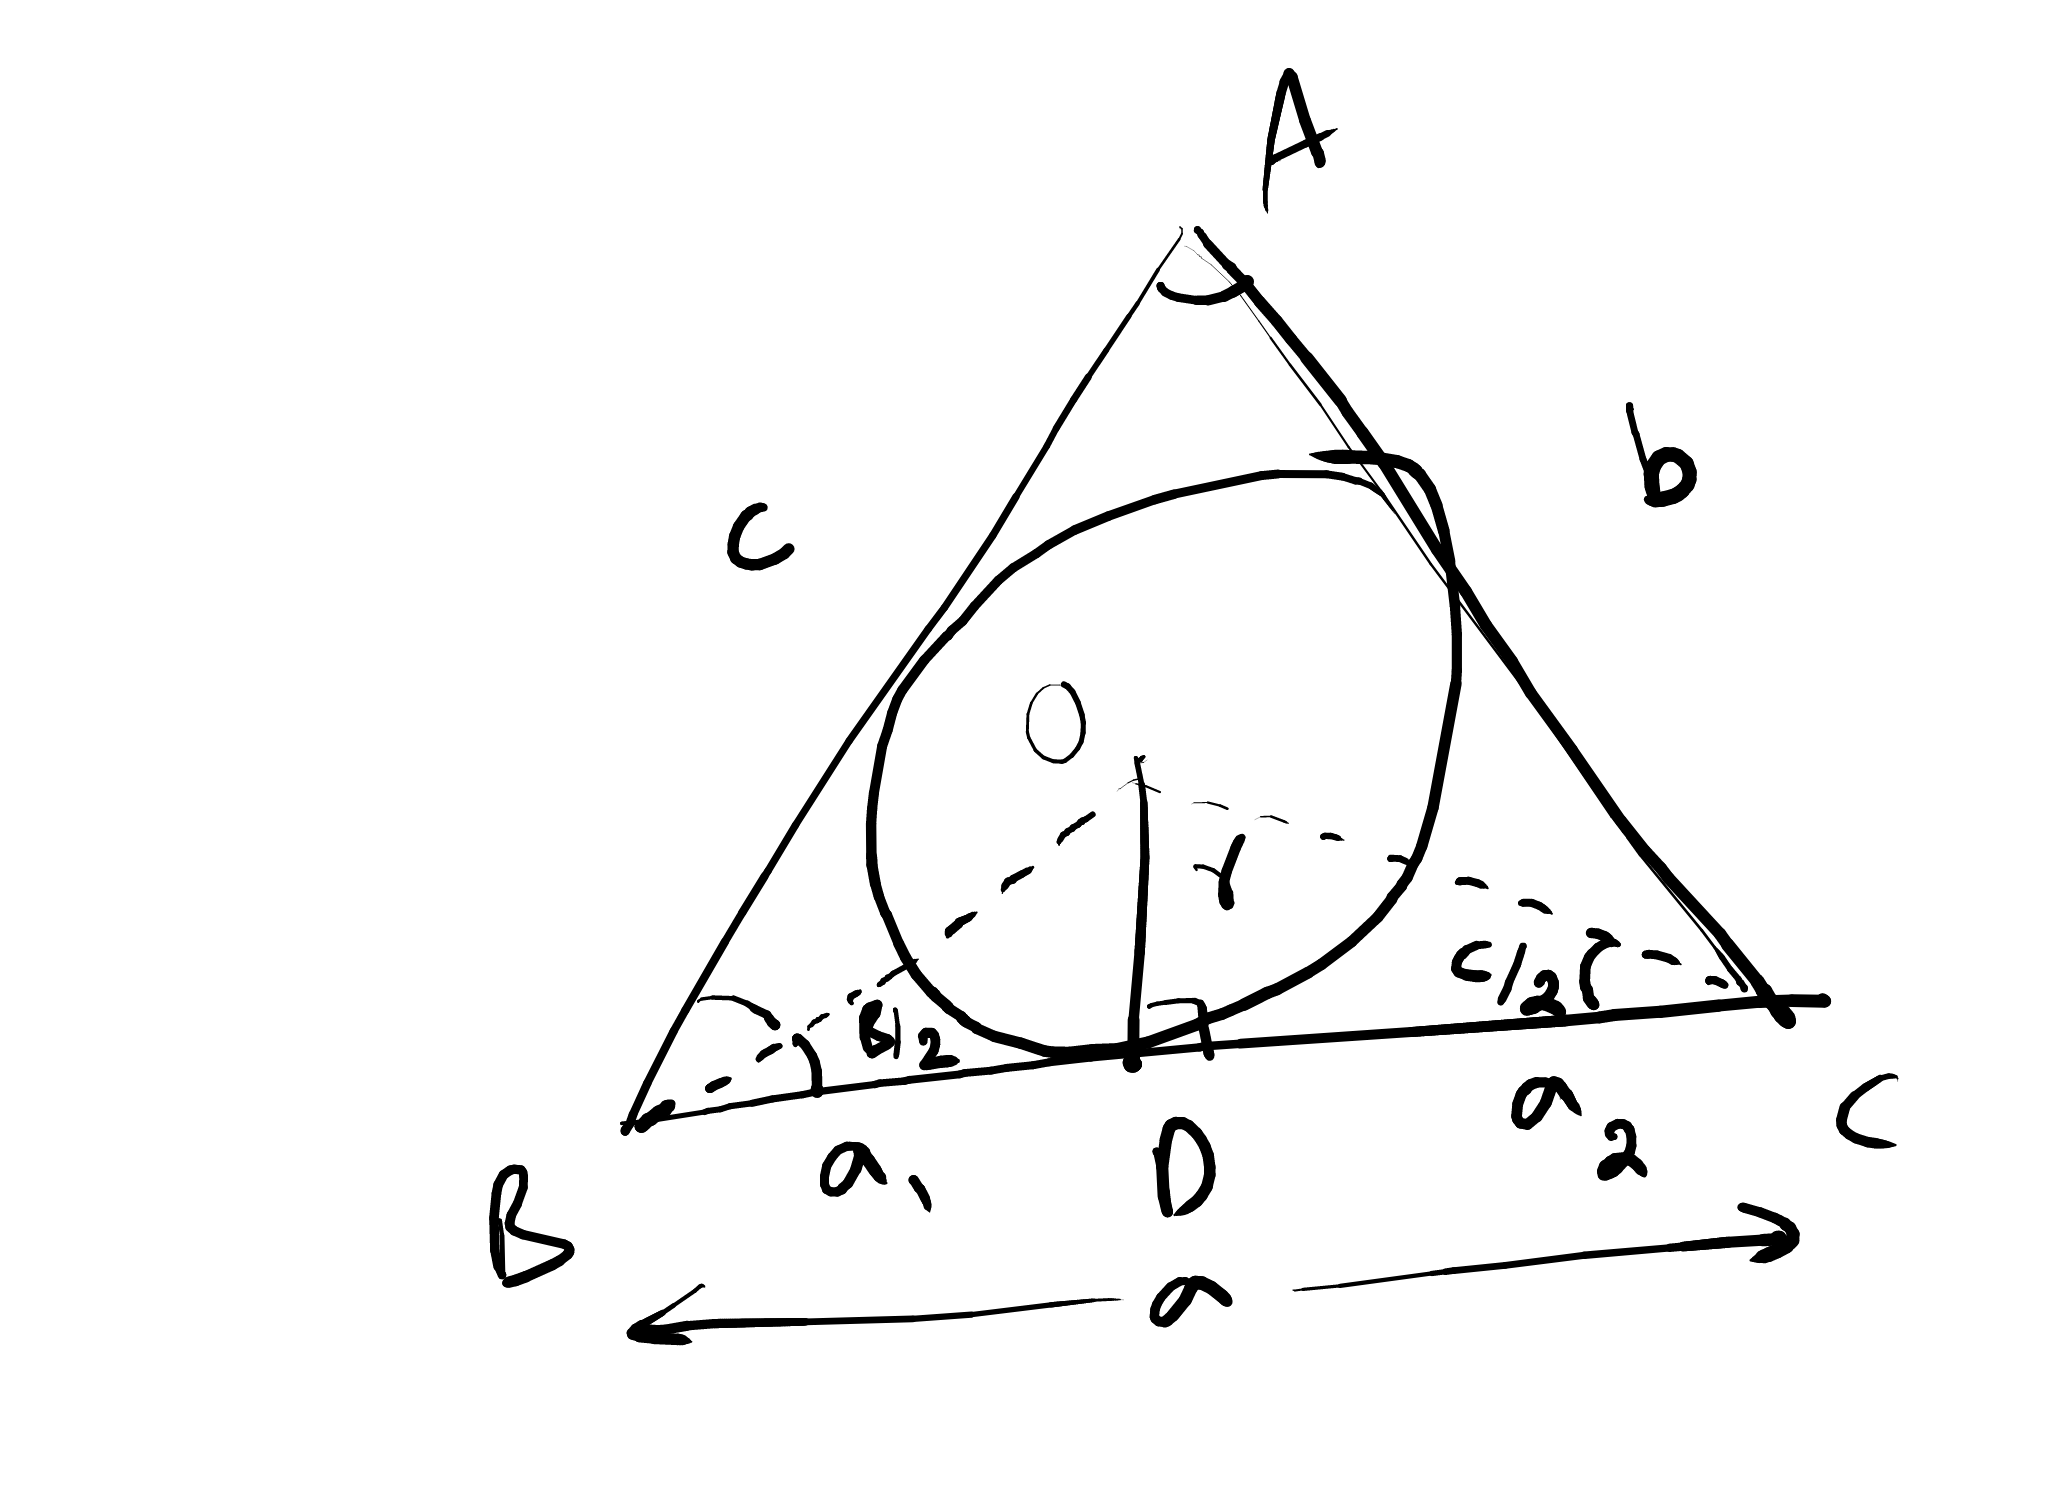
\includegraphics[width=0.6\columnwidth]{figs/ncert/circle/7.png}}
	\end{center}
	\caption{}
	\label{fig:ncert-circ-7}	
\end{figure}
\item $PQ$ is a chord of length 8 cm of a circle of radius 5 cm. The tangents at $P$ and $Q$ intersect at a point $T$. Find the length $TP$.
\item Two circles intersect at two points $A and B$. $AD$ and $AC$ are diameters to the two circles. Prove that $B$ lies on the line segment $DC$.
\item Prove that the quadrilateral formed (if possible) by the internal angle bisectors of any quadrilateral is cyclic.
\item  The perpendicular from the centre of a circle to a chord bisects the chord. 
\item  The line drawn through the centre of a circle to bisect a chord is perpendicular to the chord.
\item  There is one and only one circle passing through three non-collinear points. 
\item  Equal chords of a circle (or of congruent circles) are equidistant from the centre (or corresponding centres).
\item If a line intersects two concentric circles (circles with the same centre) with centre O at A, B, C and D, prove that AB = CD.
	\iffalse
\begin{enumerate}
\begin{figure}[!ht]
\centering
\resizebox{\columnwidth}{!}{\begin{tikzpicture}[scale = 0.5,>=stealth,point/.style={draw,circle,fill=black, inner sep=0.5pt},]
\node (O) at (0, 0)[point,label=above:$O$] {};
\node (A) at (-8.66, -5)[point,label=below:$A$] {};
\node (B) at (-4.89, -5)[point,label=below:$B$] {};
\node (C) at (4.89, -5)[point,label=below:$C$] {};
\node (D) at (8.66, -5)[point,label=below:$D$] {};
\node (M) at (0,-5)[point,label=below:$M$] {};

\draw (0,0) circle(7cm);
\draw (0,0) circle(10cm);
\draw (A) -- node[below=5pt]{}(B) -- (C) -- (D);
\draw[dotted] (O) -- node[below=5pt]{}(M);
\draw[dotted] (O) -- node[below=5pt]{}(A);
\draw[dotted] (O) -- node[below=5pt]{}(B);
\draw[dotted] (O) -- node[below=5pt]{}(C);
\draw[dotted] (O) -- node[below=5pt]{}(D);

\tkzMarkRightAngle[fill=blue!20, mark=|](O,M,B)

\end{tikzpicture}}
\caption{}
\label{fig:8.5.40_circle_1}	
\end{figure}

\item  {\em Construction: } See Fig. \ref{fig:8.5.40_circle_1}.	 The input parameters are
\begin{align}
\vec{O} &= \myvec{0\\0},
\vec{A} &= r_1\myvec{\cos \theta_1\\ \sin \theta_1}
\vec{D} &= r_2\myvec{\cos \theta_2\\ \sin \theta_2}
\end{align}
The two concentric circles  with centre $\vec{O}$ and radii $r_1$ and $r_2$ are drawn.

\subitem The equation of $AD$ is 
\begin{align}
\label{eq:8.1.40_line}
\vec{x} = \vec{A} + \lambda \brak{\vec{A}-\vec{D}}
\end{align}
Points $\vec{B}$ and $\vec{D}$ are obtained as the intersection of $AB$ and the circle with equation
\begin{align}
\label{eq:8.1.40_circle}
\norm{\vec{x}}^2 = r_2^2
\end{align}
From \eqref{eq:8.1.40_circle}
and \eqref{eq:8.1.40_circle}, 
\begin{align}
\norm{\vec{A} + \lambda \brak{\vec{A}-\vec{D}}}^2 = r_2^2
\end{align}
\begin{multline}
\lambda^2\norm{\vec{A}-\vec{D}}^2 + 2\lambda \vec{A}^T\brak{\vec{A}-\vec{D}} 
\\
+ \norm{\vec{A}}^2 -r_2^2 =0
\label{eq:8.1.40_quad}
\end{multline}
Solving the above quadratic equation yields two values for $\lambda$ yielding $\vec{B}$ and $\vec{C}$.  
\begin{align}
\vec{M} = \frac{\vec{B}+\vec{C}}{2}
\end{align}


\item {\em Proof: } In Fig. \ref{fig:8.5.40_circle_1}, 
\begin{align}
\triangle OMB \cong \triangle OMC
\\
\triangle OMA \cong \triangle OMD
\end{align}
resulting in 
\begin{align}
AM = DM
\\
BM = CM
\\
\implies AB = CD
\end{align}

\end{enumerate}
\fi
\item A chord of a circle is equal to the radius of the
circle. Find the angle subtended by the chord at
a point on the minor arc and also at a point on the
major arc.
\item If diagonals of a cyclic quadrilateral are diameters of the circle through the vertices of
the quadrilateral, prove that it is a rectangle.
\item If the non-parallel sides of a trapezium are equal, prove that it is cyclic.
	\iffalse
\begin{enumerate}

\begin{figure}[!ht]
\centering
\resizebox{\columnwidth}{!}{\begin{tikzpicture}[scale=1.5,>=stealth,point/.style={draw,circle,fill = black,inner sep=0.5pt},]
      
%Labeling points
\node (A) at (0, 0)[point,label=below left:$A$] {};
\node (B) at (5, 0)[point,label=below right:$B$] {};
\node (C) at (3.9, 3)[point,label=above right:$C$] {};
\node (D) at (1.1, 3)[point,label=above left:$D$] {};
\node (P1) at (1.1, 0)[point,label=below right:$P_1$] {};
\node (P2) at (3.9, 0)[point,label=below left:$P_2$] {};
\node (O) at (2.5, 0.79)[point,label=below:$O$]{};

%Drawing quad ABCD
\draw (A) -- node[below=6pt]{$b$}(B) -- (C) -- (D) -- (A);
\draw[dotted] (D) -- node[right = 7pt]{$h$}(P1)(P2)--(C);
\draw[dotted] (O) circle(2.62);
%marking line segment
\tkzMarkSegments[mark=|,size=6pt](A,D C,B)
\tkzMarkSegments[mark=s||,size=6pt](P1,D C,P2)

%marking angles
\tkzMarkAngle[fill=orange!40,size=0.5cm,mark=](P1,A,D)
\tkzMarkAngle[fill=orange!40,size=0.5cm,mark=](D,C,B)
\tkzMarkRightAngle[fill=blue!20](D,P1,A)
\tkzMarkRightAngle[fill=blue!20](C,P2,B)
\tkzLabelAngle[pos=0.75](P1,A,D){$\theta$}
\tkzLabelAngle[pos=0.75](D,C,B){$\alpha$}

\end{tikzpicture} }
\caption{}
\label{fig:8.5.43_trapezium}	
\end{figure}
%
\item {\em Construction: }See Fig. \ref{fig:8.5.43_trapezium}
The input parameters are
\begin{align}
\vec{A} &=\myvec{0\\0},
\vec{B} &= \myvec{b\\0}, \label{eq:8.5.43_constr_b}
\\
\vec{C} &= \myvec{b - h\cot{\theta}\\h}\label{eq:8.5.43_constr_c}\\ 
\vec{D} &= h\myvec{\cot{\theta}\\ 1}\label{eq:8.5.43_constr_d}	\end{align}
%
which are sufficient to draw the trapezium.  The circumcircle of $\triangle ABC$ is then drawn.  This circle passes through $\vec{D}$.

From \eqref{eq:8.5.43_constr_b} - \eqref{eq:8.5.43_constr_d}
\begin{align}
\vec{B} - \vec{A} &= \myvec{b\\0}\label{eq:8.5.43_dir1}\\
\vec{D} - \vec{C} &= \myvec{2h\cot{\theta}-b\\0}\label{eq:8.5.43_dir2}\\
\vec{D} - \vec{A} &= \myvec{h\cot{\theta}\\h}\label{eq:8.5.43_dir3}\\
\vec{B} - \vec{C} &= \myvec{h\cot{\theta}\\-h}\label{eq:8.5.43_dir4}
\end{align}

Finding the scalar products:
\begin{align}
\brak{\vec{D} - \vec{A}}^T\brak{\vec{B} - \vec{A}} &= \norm{\vec{D}-\vec{A}} 
\norm{ \vec{B}-\vec{A}} \cos{\theta}\label{eq:8.5.43_scalar1}\\
\brak{\vec{D} - \vec{C}}^T\brak{\vec{B} - \vec{C}} &= \norm{\vec{D}-\vec{C}} 
\norm{ \vec{B}-\vec{C}} \cos{\alpha}\label{eq:8.5.43_scalar2}
\end{align}

Dividing \eqref{eq:8.5.43_scalar2} with \eqref{eq:8.5.43_scalar1},
\begin{align}
\frac{\brak{\vec{D} - \vec{A}}^T\brak{\vec{B} - \vec{A}}}{\brak{\vec{D} - \vec{C}}^T\brak{\vec{B} - \vec{C}}} &= \frac{\norm{\vec{D}-\vec{A}}\ 
\norm{ \vec{B}-\vec{A}} \cos{\theta}}{\norm{\vec{D}-\vec{C}} 
\norm{ \vec{B}-\vec{C}} \cos{\alpha}}\label{eq:8.5.43_scalar3}
\end{align}\\
$\because \norm{ \vec{D} - \vec{A} } = \norm{ \vec{B} - \vec{C}} $, \eqref{eq:8.5.43_scalar3} can be simplified to the form
\begin{align}
\frac{\brak{\vec{D} - \vec{A}}^T\brak{\vec{B} - \vec{A}}}{\brak{\vec{D} - \vec{C}}^T\brak{\vec{B} - \vec{C}}} &= \frac{\norm{ \vec{B}-\vec{A}} \cos{\theta}}{\norm{\vec{D}-\vec{C}}cos{\alpha}}
\end{align}
%
Substituting values from \eqref{eq:8.5.43_dir1}, \eqref{eq:8.5.43_dir2}, \eqref{eq:8.5.43_dir3} and \eqref{eq:8.5.43_dir4}:
\begin{align}
\frac{bh\cot{\theta}}{\brak{2h\cot{\theta}-b}h\cot{\theta}} &= \frac{b\cos{\theta}}{b-2h\cot{\theta}}\\
\implies\cos{\alpha} &= -\cos{\theta}\\
\implies \alpha + \theta &= 180\degree
\end{align}

$\therefore ABCD$ is a cyclic quadilateral.

\end{enumerate}
\fi

\item Two circles intersect at two points $B$ and $C$.
Through $B$, two line segments $ABD$ and $PBQ$
are drawn to intersect the circles at $A, D$ and $P$,
$Q$ respectively. Prove that
$\angle ACP = \angle QCD$.
\item If circles are drawn taking two sides of a triangle as diameters, prove that the point of
intersection of these circles lie on the third side.
\item Prove that the line of centres of two intersecting circles subtends equal angles at the
two points of intersection.
\item Let the vertex of an angle $ABC$ be located outside a circle and let the sides of the angle
intersect equal chords $AD$ and $CE$ with the circle. Prove that $\angle ABC$ is equal to half the
difference of the angles subtended by the chords $AC$ and $DE$ at the centre.
\item Prove that the circle drawn with any side of a rhombus as diameter, passes through
the point of intersection of its diagonals.
\item $ABCD$ is a parallelogram. The circle through $A, B$ and $C$ intersect $CD$ (produced if
necessary) at $E$. Prove that $AE = AD$.
\item $AC$ and $BD$ are chords of a circle which bisect each other. Prove that (i) $AC$ and $BD$ are
diameters, (ii) $ABCD$ is a rectangle.
\item Bisectors of angles $A, B$ and $C$ of a $\triangle ABC$ intersect its circumcircle at $D, E$ and
$F$ respectively. Prove that the angles of the $\triangle DEF$ are $90\degree – \frac{A}{2}, 90\degree – \frac{B}{2}$ and $90\degree – \frac{C}{2}$.
\item Two congruent circles intersect each other at points A and B. Through A any line segment PAQ is drawn so that $P, Q$ lie on the two circles. Prove that $BP = BQ$.
\item In any $\triangle ABC$, if the angle bisector of $\angle A$ and perpendicular bisector of $BC$ intersect, prove that they intersect on the circumcircle of the $\triangle ABC$.
%
%
\item Prove that in two concentric circles, the chord of the larger circle, which touches the smaller circle, is bisected at the point of contact.
%
%
%
     	\item If a circle is inscribed in a right angled triangle $ABC$ right angled at $\vec{B}$, show that the diameter of the circle is equal to $AB+BC-AC$.
\item  There is one and only one circle passing through three non-collinear points. 
\item Chords equidistant from the centre  of a circle  are equal.
\item  If a line segment joining two points subtends equal angles at two other points lying on the same side of the line containing the line segment, the four points lie on a circle. 
	\iffalse
\begin{enumerate}
\begin{figure}[!ht]
\centering
\resizebox{\columnwidth}{!}{	\begin{tikzpicture}
[scale=2,>=stealth,point/.style={draw,circle,fill = black,inner sep=0.5pt},]

%Triangle sides
\def\a{5}
\def\b{6}
\def\c{4}
\def\R{3.023715784073818}

%Coordinates of A
%\def\p{0.5}
\def\p{((\a^2+\c^2-\b^2)/(2*\a))}
\def\q{{sqrt(\c^2-\p^2)}}

\def\x{((\a^2+\b^2-\c^2)/(2*\a))}
\def\y{{sqrt(\b^2-\x^2)}}

%Labeling points
%\node (A) at ($({((\a^2+\c^2-\b^2)/(2*\a))},{sqrt(\c^2-\x^2)} )$)[point,label=above right:$A$] {};
\node (A) at ($({((\a^2+\c^2-\b^2)/(2*\a))},{sqrt(\c^2-\p^2)} )$)[point,label=below left:$A$] {};
\node (B) at (0, 0)[point,label=below left:$B$] {};
\node (C) at (\a, 0)[point,label=below right:$C$] {};
\node (D) at ($({((\a^2+\b^2-\c^2)/(2*\a))},{sqrt(\b^2-\x^2)} )$)[point,label=below left:$D$] {};
%\node (E) at ($({(\a)}, {((\a)/((\a^2+\b^2-\c^2)/(2*\a))*(sqrt(\c^2-\p^2))})$)[point,label=below right:$E$] {};
%Circumcentre

\node (O) at (2.5,1.70084013)[point,label=above right:$O$] {};

%Drawing triangle ABC
\draw (A) -- node[left] {$\textrm{c}$} (B) -- node[below] {$\textrm{a}$} (C) -- node[above,yshift=2mm] {$\textrm{b}$} (A);

\draw (D) -- node[left] {$\textrm{e}$} (B);
\draw (D) -- node[left] {$\textrm{d}$} (C);

%\draw[dashed] (E) -- node[left] {$\textrm{}$} (B);
%\draw[dashed] (E) -- node[left] {$\textrm{}$} (C);
%Drawing OA, OB, OC
%\draw (O) -- node[left] {$\textrm{R}$} (A);
%\draw (O) -- node[below] {$\textrm{R}$} (B);
%\draw (O) -- node[below] {$\textrm{R}$} (C);
\draw (O) circle (\R);

%\tkzMarkAngle[fill=blue!50,size=.3](C,B,A)
%\tkzMarkAngle[fill=blue!50,size=.3](O,C,B)


%\tkzMarkAngle[fill=red!50](O,A,C)
\tkzMarkAngle[fill=red!50,size=.3](B,D,C)
%\tkzMarkAngle[fill=red!50,size=.3](B,E,C)

\tkzMarkAngle[fill=orange!50,size=.3](B,A,C)
%\tkzMarkAngle[fill=orange!50,size=.3](O,B,A)
\tkzMarkAngle[fill=red!50,size=.3](B,D,C)
\tkzMarkAngle[fill=red!50,size=.3](C,B,D)
\tkzMarkAngle[fill=red!50,size=.3](D,C,B)
%\tkzLabelAngle[pos=0.5](A,C,B){$\theta_1$}
%\tkzLabelAngle[pos=0.5](O,B,C){$\theta_1$}
\tkzLabelAngle[pos=0.5](B,D,C){$\theta_2$}
%\tkzLabelAngle[pos=0.5](B,E,C){$\theta_3$}

\tkzLabelAngle[pos=0.5](B,A,C){$\theta_1$}
%\tkzLabelAngle[pos=1.5](O,C,A){$\theta_3$}
\tkzLabelAngle[pos=0.5](C,B,D){$\beta_2$}
\tkzLabelAngle[pos=0.5](D,C,B){$\alpha_2$}

	
	\end{tikzpicture}
	}
\caption{ }
\label{fig:8.5.13_C_circle}	
\end{figure}
%
\item {\em Construction: }See Fig. \ref{fig:8.5.13_C_circle}.  The input parameters are
% 
\begin{align}
\vec{A} &= \myvec{p \\ q}
\\
\vec{B} &= \myvec{0 \\ 0}
\\
\vec{C} &= \myvec{a\\ 0} 
\end{align}
\subitem $\theta_1$ is obtained using
%
\begin{align}
\cos{\theta_1} = \frac{\brak{\vec{A}-\vec{B}}^T\brak{\vec{A}-\vec{C}}}{\norm{\vec{A}-\vec{B}}\norm{\vec{A}-\vec{C}}}
\end{align}
\subitem Let 
\begin{align}
\vec{D} &= b\myvec{\cos \beta_2\\ b \sin \beta_2} 
\label{eq:8.5.13_D}
\end{align}
From the given information, $\theta_2 = \theta_1$
\begin{align}
\implies \frac{b}{\sin\brak{\theta_2 + \beta_2}} = \frac{a}{\sin \theta_2}
\label{eq:8.5.13_b}
\end{align}
%
Choosing an appropriate value of $\beta_2$, $b$ and $\vec{D}$ can be obtained from \eqref{eq:8.5.13_D} and \eqref{eq:8.5.13_b} respectively.
\subitem The circumcircle of $\triangle ABC$ can then be drawn and it can be verified that $\vec{D}$ lies on it.

\item {Proof: } Let 
\begin{align}
\vec{O} = \myvec{0\\0}
\end{align}
%
be the circumcentre of $\triangle ABC$ and let $r$ be the radius.  Assuming that
\begin{align}
\label{eq:8.5.13_A}
\vec{A} &= r\myvec{\cos \theta_1\\\sin\theta_1},
\vec{B} = r\myvec{\cos \theta_2\\\sin\theta_2}
\\
\vec{C} &= r\myvec{\cos \theta_3\\\sin\theta_3},
\vec{D} = k\myvec{\cos \theta_4\\\sin\theta_4}
\label{eq:8.5.13_Dp}
\end{align}
in Fig. \ref{fig:8.5.13_C_circle}, from the given information
\begin{align}
 \frac{\brak{\vec{A}-\vec{B}}^T\brak{\vec{A}-\vec{C}}}{\norm{\vec{A}-\vec{B}}\norm{\vec{A}-\vec{C}}} = 
 \frac{\brak{\vec{D}-\vec{B}}^T\brak{\vec{D}-\vec{C}}}{\norm{\vec{D}-\vec{B}}\norm{\vec{D}-\vec{C}}} 
\label{eq:8.5.13_inner}
\end{align}
\begin{multline}
\because \brak{\vec{A}-\vec{B}}^T\brak{\vec{A}-\vec{C}} = \norm{\vec{A}}^2 - \vec{A}^T\vec{B}
\\
- \vec{B}^T\vec{A}+ \vec{B}^T\vec{C}
\label{eq:8.5.13_inner_expand}
\end{multline}
from \eqref{eq:8.5.13_A}-\eqref{eq:8.5.13_Dp}, \eqref{eq:8.5.13_inner_expand} can be expressed as
\begin{multline}
r^2\lsbrak{1 - \cos \brak{\theta_1-\theta_2} }
\\
\rsbrak{-  \cos \brak{\theta_1-\theta_3}+ \cos \brak{\theta_2-\theta_3}}
\\
=  r^2\brak{1-p_{12}- p_{13}+ p_{23}}
\label{eq:8.5.13_abc_inner}
\end{multline}
which can be expressed as
\begin{multline}
2r^2\lsbrak{ \sin^2 \brak{\frac{\theta_1-\theta_2}{2}} }
\\
+
\rsbrak{  \sin \brak{\frac{\theta_1-\theta_2}{2}}\sin \brak{\frac{\theta_1+\theta_2}{2} - \theta_3}}
\\
= 2r^2 \sin \brak{\frac{\theta_1-\theta_2}{2}} 
\\
\times
\sbrak{\sin \brak{\frac{\theta_1-\theta_2}{2}}
 + \sin \brak{\frac{\theta_1+\theta_2}{2} - \theta_3}}
\\
= 4r^2 \sin \brak{\frac{\theta_1-\theta_2}{2}} 
\\
\times \sin \brak{\frac{\theta_1-\theta_3}{2}} \cos \brak{\frac{\theta_2-\theta_3}{2}}
\label{eq:8.5.13_abc_innercos}
\end{multline}
%
Similarly, 
\begin{multline}
 \brak{\vec{D}-\vec{B}}^T\brak{\vec{D}-\vec{C}} = \norm{\vec{D}}^2 - \vec{D}^T\vec{B}
\\
- \vec{B}^T\vec{D}+ \vec{B}^T\vec{C}
\end{multline}
which can be expressed using \eqref{eq:8.5.13_A}-\eqref{eq:8.5.13_Dp} as
\begin{multline}
 k^2 -rk \cos\brak{\theta_2-\theta_4}
\\
-rk \cos\brak{\theta_3-\theta_4}+r^2 \cos\brak{\theta_2-\theta_3}
\\
=  k^2 -rk p_{24}-rk p_{34}+r^2  p_{23}
\label{eq:8.5.13_inner_dexpand}
\end{multline}
%
Similarly, 
\begin{align}
\norm{\vec{A}-\vec{B}}^2 &= 2r^2\sbrak{1 -  \cos \brak{\theta_1-\theta_2} } 
\\
&= 2r^2\brak{1 - p_{12}}
\label{eq:8.5.13_inner_normab}
\\
&=2 \sin^2 \brak{\frac{\theta_1-\theta_2}{2}} 
\label{eq:8.5.13_inner_normabcos}
\\
\norm{\vec{A}-\vec{C}}^2 &= 2r^2\sbrak{1 -  \cos \brak{\theta_1-\theta_3} } 
\\
&= 2r^2\brak{1 - p_{13}}
\label{eq:8.5.13_inner_normac}
\\
&=2 \sin^2 \brak{\frac{\theta_1-\theta_3}{2}} 
\label{eq:8.5.13_inner_normaccos}
\\
\norm{\vec{D}-\vec{B}}^2 &= k^2 + r^2 - 2kr \cos\brak{\theta_2-\theta_4} 
\\
&= k^2+r^2 - 2kr p_{24}
\label{eq:8.5.13_inner_normdb}
\\
\norm{\vec{D}-\vec{C}}^2 &= k^2 + r^2 - 2kr \cos\brak{\theta_3-\theta_4} 
\\
&= k^2+r^2 - 2kr p_{34}
\label{eq:8.5.13_inner_normdc}
\end{align}
%
Substituting from \eqref{eq:8.5.13_inner_dexpand}, \eqref{eq:8.5.13_abc_inner},
\eqref{eq:8.5.13_inner_normab},
\eqref{eq:8.5.13_inner_normac},
\eqref{eq:8.5.13_inner_normdb},
\eqref{eq:8.5.13_inner_normdc}
 in \eqref{eq:8.5.13_inner}, 
\begin{multline}
\frac{r^2\brak{1-p_{12}- p_{13}+ p_{23}}}{\sqrt{2r^2\brak{1 - p_{12}}}\sqrt{2r^2\brak{1 - p_{13}}}} 
\\
= \frac{k^2 -rk p_{24}-rk p_{34}+r^2  p_{23}}{\sqrt{k^2+r^2 - 2kr p_{24}}\sqrt{k^2+r^2 - 2kr p_{34}}}
\end{multline}
which can be expressed as 
\begin{multline}
\frac{1-p_{12}- p_{13}+ p_{23}}{2\sqrt{\brak{1 - p_{12}}\brak{1 - p_{13}}}}
\\
= \frac{x^2 -x p_{24}-x p_{34}+  p_{23}}{\sqrt{\brak{x^2+1 - 2x p_{24}}\brak{x^2+1 - 2x p_{34}}}}
\label{eq:8.5.13_inner_x}
\end{multline}
upon substituting
\begin{align}
x =\frac{k}{r}.
\label{eq:8.5.13_xkr}
\end{align}
From \eqref{eq:8.5.13_abc_innercos}, \eqref{eq:8.5.13_inner_normabcos}
and \eqref{eq:8.5.13_inner_normaccos},
\begin{multline}
\frac{1-p_{12}- p_{13}+ p_{23}}{2\sqrt{\brak{1 - p_{12}}\brak{1 - p_{13}}}} 
\\
= \cos \brak{\frac{\theta_2-\theta_3}{2}}
\label{eq:8.5.13_inner_123}
\end{multline}
Similarly, it can be shown that
\begin{multline}
\frac{1-p_{24}- p_{34}+ p_{23}}{2\sqrt{\brak{1 - p_{24}}\brak{1 - p_{34}}}} 
\\
= \cos \brak{\frac{\theta_2-\theta_3}{2}}
\label{eq:8.5.13_inner_234}
\end{multline}
From \eqref{eq:8.5.13_inner_123} and \eqref{eq:8.5.13_inner_234}, \eqref{eq:8.5.13_inner_x}
can be expressed as
\begin{multline}
\frac{1-p_{24}- p_{34}+ p_{23}}{2\sqrt{\brak{1 - p_{24}}\brak{1 - p_{34}}}} 
\\
= \frac{x^2 -x p_{24}-x p_{34}+  p_{23}}{\sqrt{\brak{x^2+1 - 2x p_{24}}\brak{x^2+1 - 2x p_{34}}}}
\label{eq:8.5.13_inner_x23}
\end{multline}
It is obvious that 
\begin{align}
x = 1
\end{align}
%
is a solution of \eqref{eq:8.5.13_inner_x23}
\begin{align}
\implies k = r
\end{align}
from \eqref{eq:8.5.13_xkr}.


\end{enumerate}
\fi
\item  If sum of a pair of opposite angles of a quadrilateral is 180$\degree$, the quadrilateral is cyclic.
\end{enumerate}
